% TEMPLATE for Usenix papers, specifically to meet requirements of
%  USENIX '05
% originally a template for producing IEEE-format articles using LaTeX.
%   written by Matthew Ward, CS Department, Worcester Polytechnic Institute.
% adapted by David Beazley for his excellent SWIG paper in Proceedings,
%   Tcl 96
% turned into a smartass generic template by De Clarke, with thanks to
%   both the above pioneers
% use at your own risk.  Complaints to /dev/null.
% make it two column with no page numbering, default is 10 point

% Munged by Fred Douglis <douglis@research.att.com> 10/97 to separate
% the .sty file from the LaTeX source template, so that people can
% more easily include the .sty file into an existing document.  Also
% changed to more closely follow the style guidelines as represented
% by the Word sample file.

% Note that since 2010, USENIX does not require endnotes. If you want
% foot of page notes, don't include the endnotes package in the
% usepackage command, below.

% This version uses the latex2e styles, not the very ancient 2.09 stuff.
\documentclass[letterpaper,twocolumn,10pt]{article}
\usepackage{usenix,graphicx,lastpage,enumitem,textcomp,breqn,wasysym}
\usepackage{balance,comment,tabularx,tabu,listings}

%\usepackage[pdfborder={0 0 .1}]{hyperref}
%\usepackage[table,usenames,dvipsnames]{xcolor}
\usepackage{xspace}
\usepackage[font=small,labelfont=bf]{caption}

\usepackage[switch,pagewise]{lineno}

\usepackage[notextcomp,notext,not1]{stix}
\usepackage{fancyvrb}
\usepackage{fvextra}
\usepackage{subcaption}
\usepackage{booktabs}
\usepackage{multirow}
\usepackage{stmaryrd}
\usepackage{stix}
\usepackage{bm}
\usepackage{colortbl}
\usepackage{siunitx}
\usepackage{bold-extra}
\usepackage[skins,fitting,raster]{tcolorbox}
\usepackage{algorithmicx}
\usepackage{algpseudocode}
\usepackage{algorithm}
\usepackage{inconsolata}
\usepackage{tikz}

\setlist{topsep=3pt,itemsep=0ex,left=2ex}
\usetikzlibrary{patterns}

\usepackage[normalem]{ulem}
\usepackage[T1]{fontenc}
\usepackage{textgreek}
\usepackage{relsize}

\graphicspath{{figures/}}

\urlstyle{rm}

\usepackage{microtype}

\newcommand{\sys}{\textsc{Dash}\xspace}

\frenchspacing
%Eddie Kohler protect us

\begin{document}

%don't want date printed
\date{}

%make title bold and 14 pt font (Latex default is non-bold, 16 pt)
%\title{\Large {\sys:} orchestrating massive computations on cloud functions}
\title{\textbf{\sffamily The Paper Title}}

\author{Paper \#XX (\getpagerefnumber{beforerefs}+{\number\numexpr\getpagerefnumber{LastPage}-\getpagerefnumber{beforerefs}} pages)}

\maketitle

% Use the following at camera-ready time to suppress page numbers.
% Comment it out when you first submit the paper for review.
% \pagestyle{empty}

\begin{abstract}
%
We abstract. Lorem ipsum dolor sit amet, consectetur adipisicing elit,
sed do eiusmod tempor incididunt ut labore et dolore magna aliqua. Ut
enim ad minim veniam, quis nostrud exercitation ullamco laboris nisi
ut aliquip ex ea commodo.

\end{abstract}


\section{Introduction}
\label{sec:intro}

We introduce. Lorem ipsum dolor sit amet, consectetur adipisicing
elit, sed do eiusmod tempor incididunt ut labore et dolore magna
aliqua. Ut enim ad minim veniam, quis nostrud exercitation ullamco
laboris nisi ut aliquip ex ea commodo.


\section{Related Work}
\label{s:relwork}

We relate~\cite{spark}. Lorem ipsum dolor sit amet, consectetur
adipisicing elit, sed do eiusmod tempor incididunt ut labore et dolore
magna aliqua. Ut enim ad minim veniam, quis nostrud exercitation
ullamco laboris nisi ut aliquip ex ea commodo.


\section{Design and Implementation}
\label{s:design}

We design (Figure~\ref{fig:sample}). Lorem ipsum dolor sit amet,
consectetur adipisicing elit, sed do eiusmod tempor incididunt ut
labore et dolore magna aliqua. Ut enim ad minim veniam, quis nostrud
exercitation ullamco laboris nisi ut aliquip.

\begin{figure}[h]
  \centering
  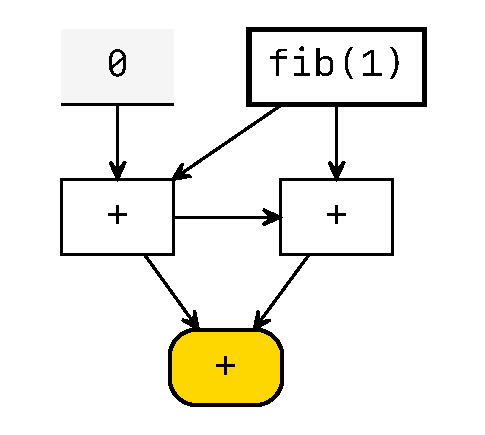
\includegraphics[width=0.5\columnwidth]{sample-figure.pdf}

  \caption{We draw. Lorem ipsum dolor sit amet, consectetur
  adipisicing elit, sed do eiusmod tempor incididunt ut labore.}

  \label{fig:sample}
\end{figure}



\section{Evaluation}
\label{sec:eval}

We evaluate. Lorem ipsum dolor sit amet, consectetur adipisicing elit,
sed do eiusmod tempor incididunt ut labore et dolore magna aliqua. Ut
enim ad minim veniam, quis nostrud exercitation ullamco laboris nisi
ut aliquip ex ea commodo consequat. Duis aute irure dolor in
reprehenderit in voluptate velit esse cillum dolore eu fugiat nulla
pariatur. Excepteur sint occaecat cupidatat non proident, sunt in
culpa qui officia deserunt mollit anim id est laborum.


\section{Conclusion}
\label{s:conclusion}

We conclude. Lorem ipsum dolor sit amet, consectetur adipisicing elit,
sed do eiusmod tempor incididunt ut labore et dolore magna aliqua. Ut
enim ad minim veniam, quis nostrud exercitation ullamco laboris nisi
ut aliquip ex ea commodo consequat. Duis aute irure dolor in
reprehenderit in voluptate velit esse cillum dolore eu fugiat nulla
pariatur.


\section*{Acknowledgments}

We thank. Lorem ipsum dolor sit amet, consectetur adipisicing elit,
sed do eiusmod tempor incididunt ut labore et dolore magna aliqua. Ut
enim ad minim veniam, quis nostrud exercitation ullamco laboris nisi
ut aliquip ex ea commodo.


%\balance

\label{beforerefs}

{
%\small
\bibliographystyle{plain}
\bibliography{paper}
}

\end{document}
